\documentclass{article}

% set font encoding for PDFLaTeX or XeLaTeX
\usepackage{ifxetex}
\ifxetex
  \usepackage{fontspec}
\else
  \usepackage[T1]{fontenc}
  \usepackage[utf8]{inputenc}
  \usepackage{lmodern}
  \usepackage{graphicx}
  \usepackage{siunitx}
\fi

% used in maketitle
\usepackage[left=3cm,right=3cm,top=3cm,bottom=3cm]{geometry}
\title{Actividad 5}
\author{Luis Aarón Cerón Ramírez}

% Enable SageTeX to run SageMath code right inside this LaTeX file.
% documentation: http://mirrors.ctan.org/macros/latex/contrib/sagetex/sagetexpackage.pdf
% \usepackage{sagetex}

\begin{document}
\maketitle
\section{Introducción}
En esta practica se llevo a cabo un analisis de datos aplicado a fenomenos meteorologicos. La actividad consistio en utilizar datos previamentente obtenidos de la actividad 4 y, darles un tratamiento para asi poder trabajar con solo las variables deseadas. Tambien se hizo una pequeña investigacion sobre los conceptos utilizados en la practica. Una vez obtidos los datos se procedio a hacer un programa para analizarlos y dar nuestras conclusiones al respecto.
\section{Conceptos fisícos}
\subsection{CAPE}
Esta son las siglas de Convective Available Potencial Energy (ó energia potencial disponible para la conveccidad), se trata de uno de los parametros convectivos mas interesantes de todos aquellos que se derivan de los modelos meteorologicos.
\newline
Se trata de un factor que determina la “Energía potencial que una parcela de aire tiene cuando alcanza el nivel de convección libre y se vuelve más cálida que el aire a su alrededor experimentando empuje ascensional hacia arriba”. Esta energía, poco a poco sufre una transformación a energía cinética del movimiento ascendente de la masa de aire que estemos analizando, por lo que se pueden obtener datos sobre velocidades de ascensos a partir de esta información.
\newline
Se trata de un parámetro que nos indica cuanta energía está disponible para la convección en caso de que esta se inicie. Por lo tanto, la consulta de este parámetro se tiene que complementar siempre con la lectura de otros campos del modelo que nos permitan determinar la probabilidad de que la convección se inicie.
\newline
Sus valores pueden ir entre 0 y unos pocos miles de J/Kg indicando un mayor grado de inestabilidad cuanto mayor es su valor.

\subsection{PW}
El agua atmosférica existe principalmente como un gas o vapor, pero breve y localmente en liquido en la lluvia, o en pequeñas gotas de agua en las nubes, o puede convertirse en sólido en la nieve, en el granizo y en los cristales de hielo de las nubes. La cantidad de vapor de agua en la atmósfera es menor que una parte en 100.000 de toda el agua de la Tierra, pero cumple una función vital en el ciclo hidrológico.
\newline
El agua precipitable es la cantidad de agua, expresada como altura o masa, que se obtendría si todo el vapor de agua contenido en una columna específica de la atmósfera, de sección transversal horizontal unitaria, se condensase y precipitase.

\section{Proceso de limpeza y filtración de datos}
Se comenzo obteniendo un script de la actividad anterior en el cual se juntaron doce archivos de datos en uno solo , en el cual se agruparon datos mensuales del 2017.
\newline
Que produce un solo archivo df2017.csv, con los renglones de variables derivadas de los datos de sondeos diarios. Con las siguientes datos:
\begin{verbatim}
$ head -13 df2017.csv

<LINK REL="StyleSheet" HREF="/resources/select.css" TYPE="text/css">

<H2>76225  Chihuahua, Chih. Observations at 00Z 01 Jan 2017</H2>

                             Station number: 76225

                            Showalter index: 1.28

    LIFT computed using virtual temperature: 0.80

                                SWEAT index: 163.35

                                    K index: 23.10

                        Totals totals index: 49.20

             CAPE using virtual temperature: 0.00

             CINS using virtual temperature: 0.00

          Bulk Richardson Number using CAPV: 0.00

  Temp [K] of the Lifted Condensation Level: 267.49

Precipitable water [mm] for entire sounding: 9.42
\end{verbatim}
El archivo contiene los datos de los diferentes lanzamientos diarios y se eliminó el resto de información.

Con una combinación del comando grep y el filtro wc aplicados al archivo df2017.csv, se determina que datos están mas completos para el 2017 de la estación seleccionada.


\section{Análisis de datos}
Se comenzo por darle un orden a los datos , lo cual nos brindaria mas facilidad al momento de trabajar con ellos.
\newline
Con ayuda de los comandos de emacs se depuraron los datos, de manera tal que se pudo dar el formato pedido en la practica, donde la primera columna será la fecha, la segunda el CAPE y la tercera el Agua precipitable (mm) y los meses: Jan, Feb, Mar, ... se reemplazaron por los números: 01, 02, 03, .... etc.
\newline
Una vez echo esto se prosiguio a usar jupyter notebook de manera que pudieramos crear los graficos necesarios para el analisis.
Los graficos obtenidos a partir de los datos son los siguientes:


\begin{figure}[H]
\centering
\includegraphics[scale=0.59]{month00z.png}
\caption{Grafica de month vs cape para 00Z}
\label{figure: mes vs cape para 00Z}
\end{figure}

\begin{figure}[H]
\centering
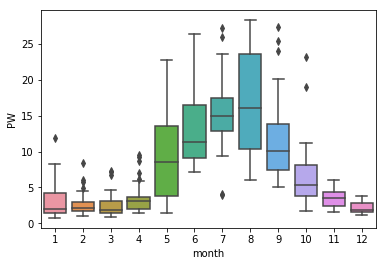
\includegraphics[scale=0.59]{pw00z.png}
\caption{Grafica de month vs pw para 00Z}
\label{figure: mes vs cape para 00Z}
\end{figure}

\begin{figure}[H]
\centering
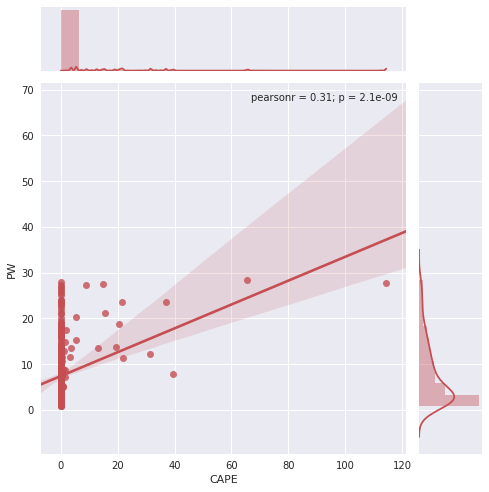
\includegraphics[scale=0.59]{pvc00z.png}
\caption{Grafica de pw vs cape para 00Z}
\label{figure: pw vs cape para 00Z}
\end{figure}

\begin{figure}[H]
\centering
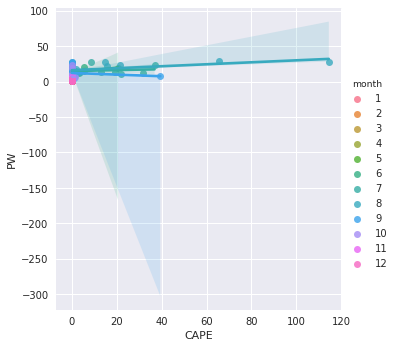
\includegraphics[scale=0.6]{pvc200z.png}
\caption{Segunda grafica de  pw vs cape para 00Z}
\label{figure: pw vs cape para 00Z}
\end{figure}

\begin{figure}[H]
\centering
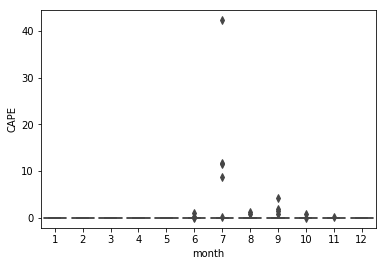
\includegraphics[scale=0.6]{month12z.png}
\caption{Segunda grafica de  pw vs cape para 12Z}
\label{figure: pw vs cape para 12Z}
\end{figure}

\begin{figure}[H]
\centering
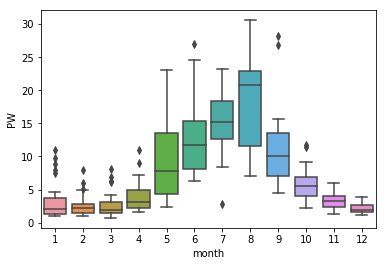
\includegraphics[scale=0.59]{pw12z.png}
\caption{Segunda grafica de  pw vs cape para 12Z}
\label{figure: pw vs cape para 12Z}
\end{figure}

\begin{figure}[H]
\centering
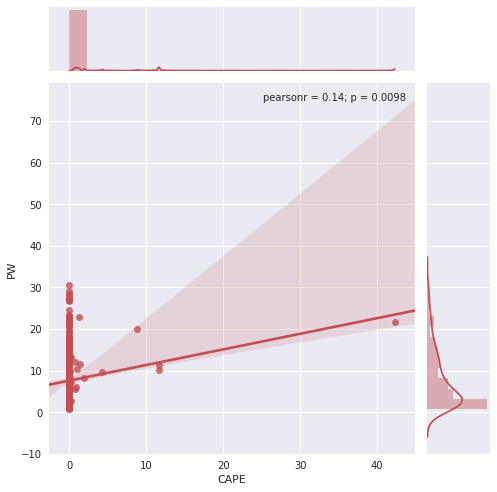
\includegraphics[scale=0.6]{pvc12z.png}
\caption{Segunda grafica de  pw vs cape para 12Z}
\label{figure: pw vs cape para 12Z}
\end{figure}

\begin{figure}[H]
\centering
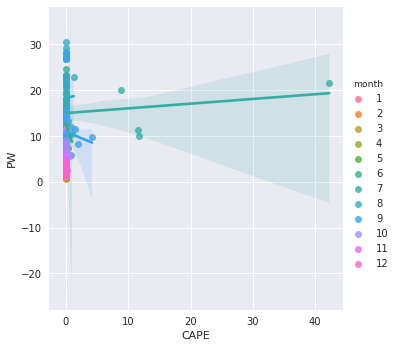
\includegraphics[scale=0.59]{pvc212z.png}
\caption{Segunda grafica de  pw vs cape para 12Z}
\label{figure: pw vs cape para 12Z}
\end{figure}


\section{Conclusión}
Como se pudo observar a la hora de manipular datos por medio de los comandos de emacs, estos facilitaron de manera muy importante el trabajo, por lo que se demostro la importancia de sino dominar los comandos si conocer las funciones basicas, ya que esto hace ahorrar mucho tiempo la limpeza de datos ára el trabajo.

\section{Apendice}

\newline
Preguntas antes de terminar:
\newline
¿Cómo se te hizo esta actividad? ¿Compleja, Difícil, Sencilla?
\newline
Una vez entendido el algoritmo que se necesitaba hacer para arreglar los datos la actividad se volvio facil
\newline
¿Qué te llamó más la atención?
\newline
La necesidad de usar comandos para ahorrar tiempo a la hora de realizar el codigo
\newline
¿Qué parte fue la que menos te interesó hacer?
\newline
El reporte, pues sigo teniendo problemas a la hora de colocar las imagenes
\newline
¿Cómo mejorarías esta actividad? ¿Qué le faltó? ¿Qué sobró?
\newline
me parecio que la actividad estaba bien hecha asi que no le agregaria nada, tal vez una pequeña introduccion a la interpretacion de graficos obtenidos pues hubo algunos gaficos que no conocia y de los cuales no puedo decir mucho
\newline
¿Hasta este punto, que te parece el uso de Jupyter para programar en Python?
\newline
Me parece un entorno muy util ademas de intuitivo puedes encontrar mucha ayuda en linea


\end{document}
